\section{Durchführung}
\label{sec:Durchführung}

In \autoref{fig:1} ist der Aufbau des Geiger-Müller-Zählrohrs inklusive 
Verstärker und Oszilloskop schematisch dargestellt.
\begin{figure}[H]
    \centering
        \centering
        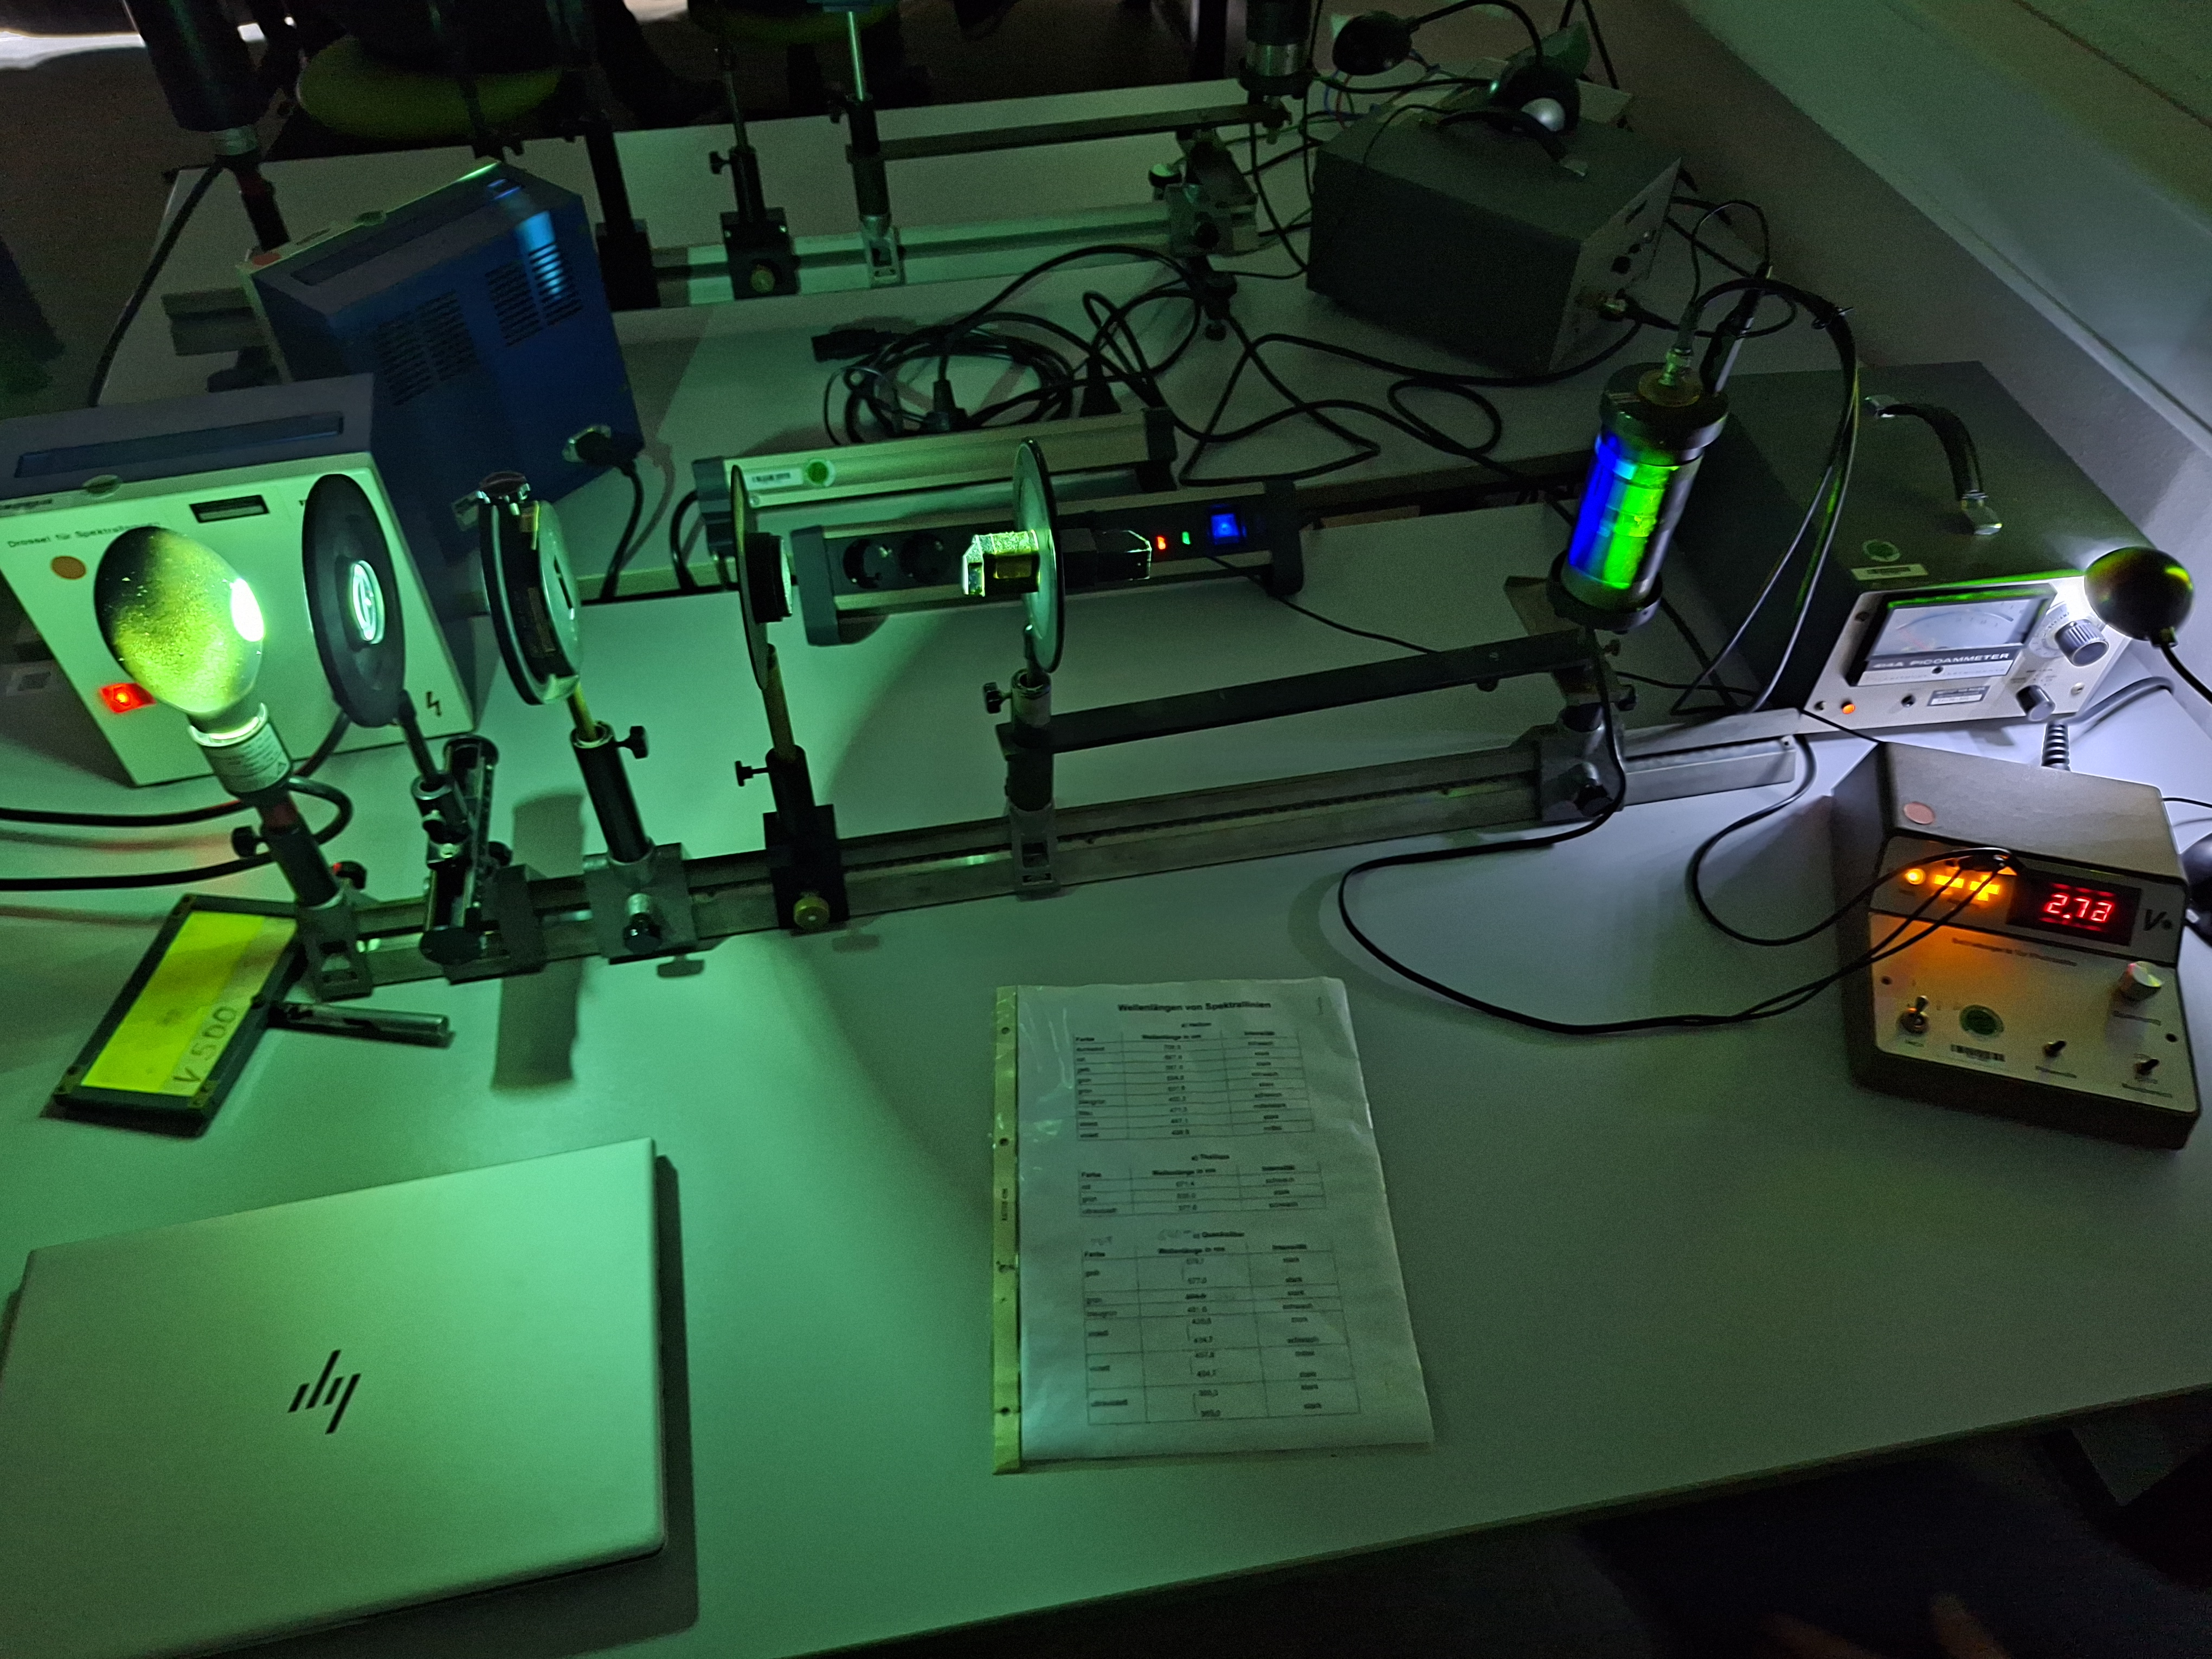
\includegraphics[width=\textwidth]{Bilder/aufbau.png}
        \caption{Skizze des Aufbaus. \cite{anleitung6}}
    \hfill
    \label{fig:1}
\end{figure}
\noindent Links ist das Geiger-Müller-Rohr mit Kathode und Anode, angeschlossen 
an ein Spannungsgerät, in der Mitte zu sehen, rechts davon befinden sich
Verstärker und schließlich der Zähler. Der angelegte Widerstand $R$ verfügt
über einen Wert im $\unit{\mega\ohm}$, sodass der Großteil der Elektronen aus
Anode in Richuntung Zähler wandern.
Ein Bild der Aufbaute nach Plan ist in \autoref{fig:2} zu finden.
\begin{figure}[H]
    \centering
        \centering
        \includegraphics[width=\textwidth]{Bilder/aufbau1.jpg}
        \caption{Versuchsaufbau nach Plan.}
    \hfill
    \label{fig:2}
\end{figure}
\noindent Während links Oszilloskop und Spannungsversorgung und rechts der 
Zähler inklusive Verstärker zu sehen sind, befindet sich das Geiger-Müller-
Zählrohr mittig in dem mit Metall abgeschirmten Bereich.

\subsection{Bestimmung der Kennlinien}
Zur Aufnahme der Kennlinien wird bei einer konstanten Messzeit von $\Delta t 
= \qty{60}{\second}$ in Abhängigkeit der angelegten Spannung bestimmt. 
Beginnend  bei einer Anfangsspannung von 300 Volt wird die Spannung schrittweise 
um $20 \unit{\volt}$ erhöht. Dieses Verfahren geht so lange, bis das Geiger-
Müller-Plateu erreicht ist. Jenes zeigt den Übergang zum Dauerentladungsbereich 
durch sprunghaften Anstieg der Zählrate auf.

\subsection{Bestimmung der Totzeit durch Oszilloskop und Zwei-Quellen-Methode}
Um die Totzeit mithilfe des Oszilloskops zu bestimmen, wird der Abstand der 
Peaks auf dem Display abgelesen. 
Für die alternative Methode werden zwei radio-aktive Quellen benötigt. Beide 
werden in der Apparatur installiert und eine spezifische Spannung gewählt. 
Zunächst wird die Anzahl der Impulse einer Probe jeweils innerhalb von 
$\Delta t = \qty{120}{\second}$ gemessen, dann von beiden gleichzeitig.